\documentclass{article} % For LaTeX2e
\usepackage{nips15submit_e,times}
\usepackage{hyperref}
\usepackage{url}
\usepackage{caption}
\usepackage{graphicx, subfigure}
\usepackage{float}
%\documentstyle[nips14submit_09,times,art10]{article} % For LaTeX 2.09


\title{Information Extraction from Textbooks \\ for Physics Knowledge}

\author{
Arman Bolat \\
ECE MS '15 \\
\texttt{abolat@andrew.cmu.edu} \\
\And
Bryan Tan \\
ECE MS '15 \\
\texttt{bstan@andrew.cmu.edu} \\
}

% The \author macro works with any number of authors. There are two commands
% used to separate the names and addresses of multiple authors: \And and \AND.
%
% Using \And between authors leaves it to \LaTeX{} to determine where to break
% the lines. Using \AND forces a linebreak at that point. So, if \LaTeX{}
% puts 3 of 4 authors names on the first line, and the last on the second
% line, try using \AND instead of \And before the third author name.

\newcommand{\fix}{\marginpar{FIX}}
\newcommand{\new}{\marginpar{NEW}}

\nipsfinalcopy % Uncomment for camera-ready version

\begin{document}

\maketitle


\begin{abstract}
The goal of this project is to build a classifier that is able to extract physics knowledge from textbooks. Information extraction of textbooks is a useful problem to tackle because of the many applications that the extracted information could be used for. In the course of this project, textbooks in the PDF will be converted to a text format, classifiers of different complexity will be tested for accuracy of determining sentences containing physics knowledge, and information will be extracted and formatted from these sentences. Training data sets will be created by extracting laws, theorems, definitions, and other knowledge in the text format textbook, and attaching any relevant material, such as context or metadata.
\end{abstract}

\section{Introduction}

As more and more information is becoming digitalized, the importance of information extraction through machine learning methods has increased. The goal of this project is to extend machine learning methods to extract physics knowledge from textbooks. In particular, this project will focus on extracting theorems, laws, and definitions relevant to Newtonian physics within a textbook. The resulting knowledge will be presented as a glossary, corresponding words and phrases with their respective definitions, formulas, or statements.

Information extraction from textbooks has a number of practical applications. For one, a problem from a textbook can be analyzed, and the relevant laws, theorems, and equations can be determined by using the knowledge extracted from textbooks, and potentially even a step by step solution for the problem could be provided by determining the relationship between different pieces of knowledge, as seen in Figure~\ref{fig:wolfram-alpha}. The extracted physics knowledge from a given textbook can also show a quick summary of the material covered in the textbook and allow for a classification of the textbook based on depth and breadth of material covered. Even more advanced would to be build a customized textbook through extracted information based on personalized needs.

\begin{figure}[t]
\centering
\subfigure{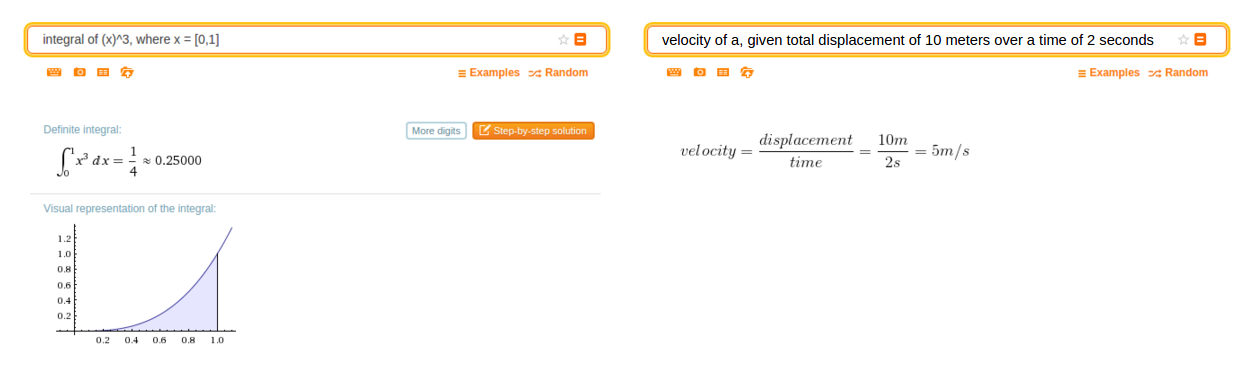
\includegraphics[width=1\textwidth]{wolframalpha.png}}
\caption{Existing Q\&A System and Potential Physics Q\&A System}
\label{fig:wolfram-alpha}
\end{figure}

The goal of this project is to extract physics knowledge from a set of textbooks.
The rest of this report is organized as follows: related works to this project will be covered in section 2, the method of creating and training the classifier will be covered in section 3, results will be covered in section 4, and conclusions drawn will be covered in section 5.

\section{Related Works}

The employment of information extraction and machine learning techniques for textbooks has not seen much work. However, there has been research into the application of knowledge extraction, such as the implementation of some of the example applications mentioned in the introduction. It is possible that the ease of access to resources that provide the information and data necessary (without the use of textbooks specifically) for such research is an explanation for the lack of research into information extraction for textbooks.

[4] explores a method of automatically solving geometry questions. To accomplish this, both the diagram and the accompanying text must be understood. A visual definition of key concepts and terms must be learned, instead of a textual definition as in this project. Through understanding diagram and text, the problem can be solved by drawing relationships between the two, using an external information source to determine the relationships between two geometry terms, such as "triangle" and "parallel", and using known information and relationships together. See Figure~\ref{fig:related-works} for an example from the paper.

[5] attempts to create a tool that is able to assess the comprehension burden, or the difficulty in understanding the textbook material. A property of well-written textbooks is that concepts are presented in sequential order, such that each concept is explained before it occurs in examples or other concepts. A textbook with high comprehension burden thus does not present concepts in sequential order. In order for this to be determined, the occurrences and definition of concepts must be found. The comprehension burden of each individual concept can then be calculated by seeing how often a concept is used before it is defined. From the comprehension burden of individual concepts, the overall comprehension burden of the textbook can be determined.

[6] enriches the learning experience by automatically finding relevant images for each chapter. In order to do so, key nouns, phrases, and ideas must be found, as well as corresponding relevant images for the found terms. This is similar to this project in that key ideas must be determined, but does not attempt to establish a relationship between key ideas. [7] also applies similar techniques to find key concept phrases, and then determines if these sections of the book are well written.

[1] aims to create a concept hierarchy of a textbook. Concepts are identified and extracted by using Wikipedia as a resource. This is very similar to this project - the intermediate goal of extracting concepts is shared, albeit without the use of an external source as a direct reference. The relationships between the identified concepts are then explored, and the hierarchy of the textbook is formed from this information. See Figure~\ref{fig:related-works} for the process used. The end goal is more complex in the hierarchy extraction paper, as the relationship between concepts must be determined. [2], a system designed at Penn State, extends upon research done in concept hierarchy extraction to automatically create open versions of textbooks by updating the textbook content through online resources such as Wikipedia. Users can specify the concepts that they want to have included in the generated textbook, and the concept hierarchy information enables the system to include information and concepts that are necessary to the understanding of the user’s selected topics.

\begin{figure}[t]
\centering
\subfigure{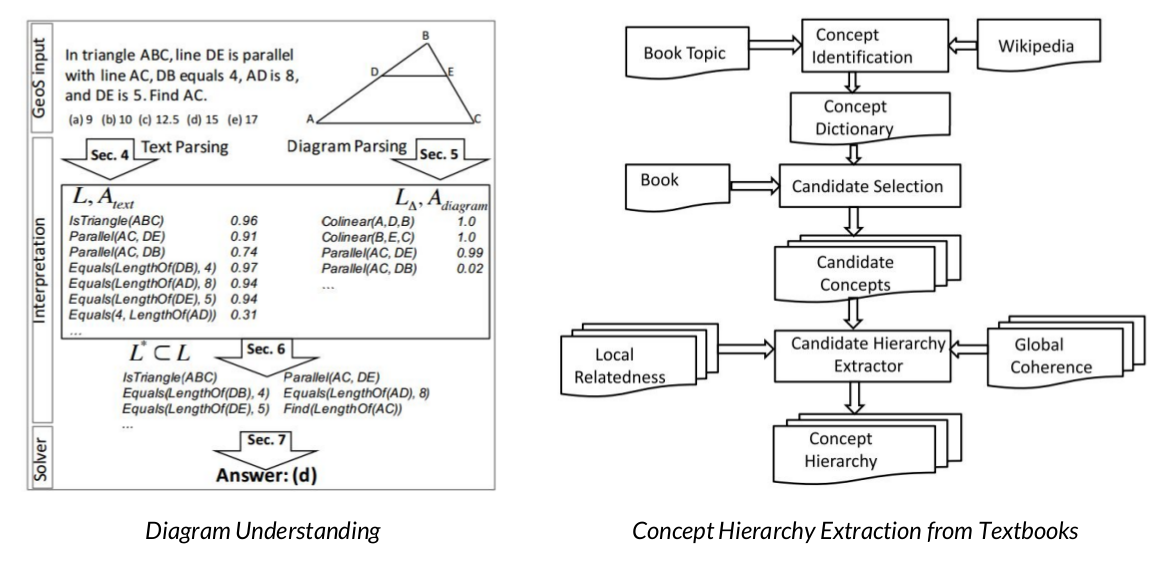
\includegraphics[width=1\textwidth]{relatedworks.png}}
\caption{Overview for Diagram Understanding and Concept Hierarchy Extraction from Textbooks}
\label{fig:related-works}
\end{figure}

\section{Method}

\begin{figure}[H]
\centering
\subfigure{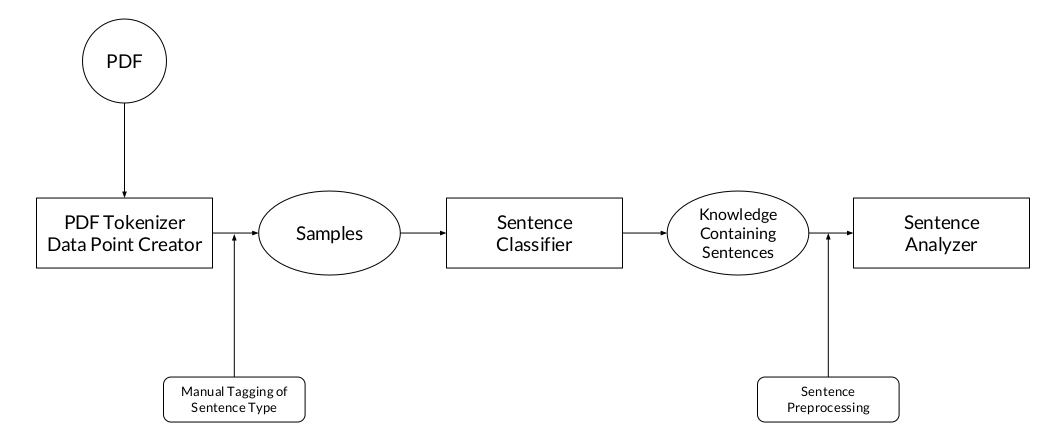
\includegraphics[width=1\textwidth]{process.png}}
\caption{Different Components of Textbook Information Extraction}
\label{fig:process}
\end{figure}
%\noindent%
%\begin{minipage}{\linewidth}% to keep image and caption on one page
%\makebox[\linewidth]{%        to center the image
%  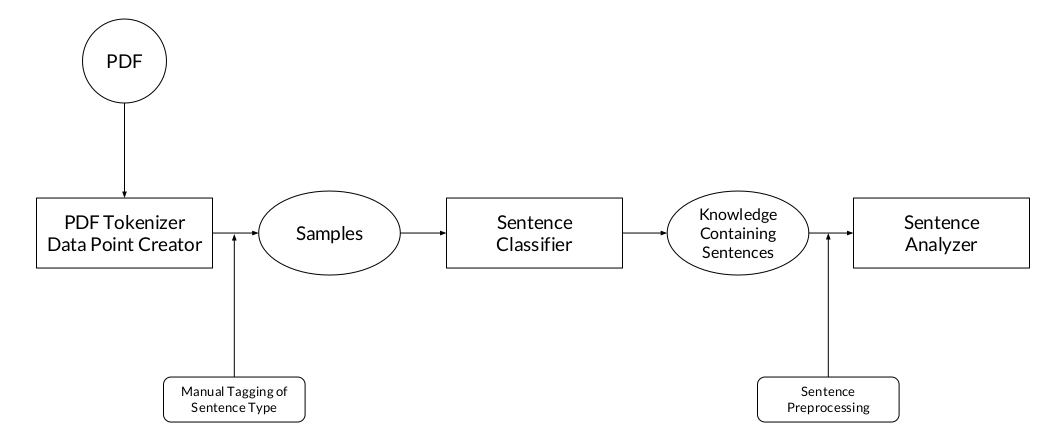
\includegraphics[keepaspectratio=true,scale=0.6]{process.png}}
%\captionof{figure}{Different Components of Textbook Information Extraction}
%\label{fig:process}%      only if needed  
%\end{minipage}

\subsection{Training Data Extraction}

It is important to generate the training data with the appropriate set of features that would be analyzed by the classifier. The training data used for this project will be extracted from the physics textbooks from [3], and specifically the chapters on the Newtonian physics. For each sentence in the textbooks, a single training data point will be created, which will be represented as a sample object. The sample object will include all the features that could be used by the classifier. A sample object can be found in Figure~\ref{fig:data-example}.

Specifically, each sample object will include:
\begin{itemize}
	\item the sentence itself
	\item the sentence before the current sentence
	\item the sentence following the current sentence
	\item the type or label of the sample object (theory/law, definition, or none)
	\item any other relevant information, such as if the sentence is bold or if the sentence contains a mathematical formula or expression
\end{itemize}

The classifiers will be using not only the content of the sentence but also the context of where the sentence is located as well as the metadata of the sentence. By including a greater number of features, a more general training data set for different classifiers can be created. Since different classifiers might be considering different set of features, it is better to include all possible features which decide if a particular sentence is a piece of physics knowledge or just a regular sentence.

Determining the start and end of each sentence is a difficult problem, and often can be a machine learning problem on its own. In order to avoid creating a tokenizer that is overly specific to the textbook used for training, many of the training samples contain multiple sentences or have some formatting issue. Watermarks, titles and headers, and text accompanying figures all can be mistaken as part of the main content of the textbook. This is an area of improvement that will not be handled very thoroughly and accurately for the sake of the scope of this project.

\begin{figure}[H]
\centering
\subfigure{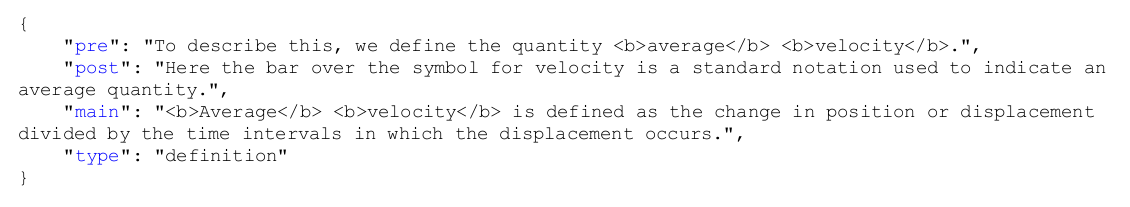
\includegraphics[width=1\textwidth]{dataexample.png}}
\caption{Sample object}
\label{fig:data-example}
\end{figure}

\subsection{Naive Bayes Implementations}

After the sentence extractor has been created, the classification part of the project will begin with implementing a simple Naive Bayes classifier and compare the accuracy by gradually increasing the number of features the classifier considers. Specifically, a classifier implementing a bag-of-words model which only looks at the words used in the sentence will be created. After the completion of the simple classifier, the implementation will be modified to account for the sentence metadata as well. The final Naive Bayes implementation will take into account all features of a sentence in order to classify it. Multiple iterations will be made to identify important features for use in future implementations.

\subsection{Classifier Selection with Machine Learning Toolkit}

After creating multiple Naive Bayes implementations and identifying important features, a machine learning toolkit will be used to further determine features, process data, and select and refine a classifier that will be used to extract sentences containing physics knowledge. Various tools in the machine learning toolkit, such as undersampling and oversampling, automatic feature selection, and boosting will be employed to arrive at a final classifier.

\subsection{Information Extraction from Relevant Sentences}

Using the final classifier obtained in the previous step, testing data will be processed to determine sentences relevant to physics knowledge. A second classifier will be used to extract information from these sentences. Information will be formatted and presented in a consistent manner, so as to provide future research with a useful interface for viewing the physics knowledge found in a textbook. In specific, Conditional Random Fields will be used to predict the structure of the knowledge sentences and derive the relationship between the different physics terms.

\begin{figure}[H]
\centering
\subfigure{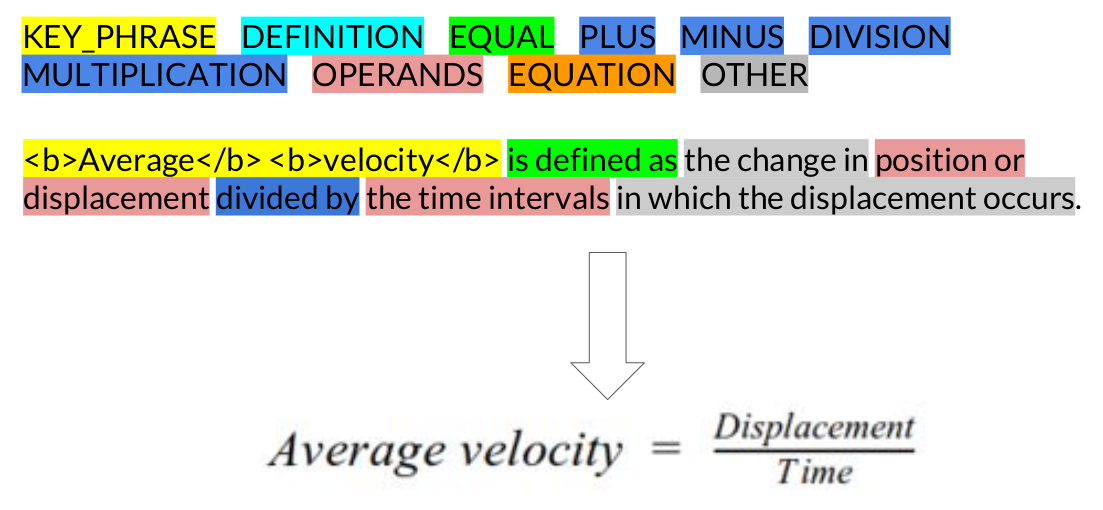
\includegraphics[width=0.6\textwidth]{crfexample.png}}
\caption{CRF Tagging of Sentence}
\label{fig:crf-example}
\end{figure}

\section{Results}

For the first half of the project, multiple Naive Bayes implementations were created. The implementations were created through an iterative process, each new implementation improving on the previous iteration by removing unnecessary features and adding relevant features. The resulting classification recall rate can be seen in tables 1 and 2 below. The recall score was used as the primary metric of accuracy due to the nature of the project - results from this sentence classification are to be analyzed and physics knowledge and relationships are drawn from the classified sentences, so for the effectiveness of the final analysis through CRFs, it is better to keep false positives to a minimum.

\subsection{Simple Bag-of-words Approach}

The initial approach of using a bag-of-words model seemed fairly successful with a training data recall of 81.70\% and a testing data recall of 71.72\%. However, upon inspection, it was clear that this initial approach was failing: for the testing data, the recall for general (non-knowledge) sentences was 95.58\%, but the recall for knowledge sentences was only 3.17\%. This indicated that the bag-of-words model had a feature set that was too large to effectively classify the sentences, which all had a relatively small number of features, or words, compared to other problems solved by a bag-of-words approach.

The poor results highlighted areas of interest worth tackling to improve the classification accuracy: adding more weight to important and distinguishing phrases or words, and taking into account the other features of the text (namely, the existence of bolded words). The script used to split textbook chapters up into sentences was also further improved to handle edge cases more effectively.

\subsection{Bag-of-words Approach with Weighting}

After implementing the changes to fix problems pointed out in the initial approach, the new classifier improved in training data knowledge sentence classification recall, going from 17.83\% to 21.99\%, but regressed in testing data knowledge sentence classification recall, going from 3.17\% to 1.35\%. The weighting did not improve the classification accuracy, as the size of the vector of indicator features was still too large in comparison to the size of the sample sentences.

\subsection{Naive Bayes with Key Phrases}

The results of the second iteration showed that a bag-of-words approach would not work, even after adding weights and accounting for different features. Thus, instead of using a bag-of-words approach, a few key phrases such as "is defined" and "is called" were selected and used as the indicator features, along with the presence of bolded words. The result of the simpler classifiers were substantially better: 35.29\% classification recall for testing data knowledge sentences. After looking through the misclassified examples, it became clear that the training data itself actually had many misclassified samples. After going through the data set to look for any missed definitions, the classification recall rose to 76.47\%. The features used in this implementation and their respective frequencies can be seen in Table~\ref{tab:word-prob}.

The precision and F1 scores of the final Naive Bayes classifier can be seen in Table~\ref{tab:nbfinal-results}. The low precision indicates that there are a number of knowledge-containing sentences that are not being classified as such correctly. This is due to the high reliance on key phrases in classifying the sentence. By focusing on these key phrases, this classifier is unable to learn new knowledge sentences that vary from the existing samples.

\begin{center}
\captionof{table}{Comparison of classification accuracies for training set data} \label{tab:nb-training} 
\begin{tabular}{ |c||c|c|c| }
	\hline
	\multicolumn{4}{|c|}{Training Data Set Classification Accuracies} \\
	\hline
	Classifier & Knowledge Sentence & General Sentence & Overall \\
	\hline
	Simple bag-of-words & 17.83\% & 98.40\% & 81.70\% \\
	Weighted bag-of-words & 21.99\% & 98.01\% & 86.69\% \\
	Naive Bayes with Key Phrases & 43.06\% & 96.68\% & 95.66\% \\
	Naive Bayes, fixed data set & 86.11\% & 96.55\% & 96.45\% \\
	\hline
\end{tabular}

\captionof{table}{Comparison of classification accuracies for testing set data} \label{tab:nb-testing} 
\begin{tabular}{ |c||c|c|c| }
	\hline
	\multicolumn{4}{|c|}{Testing Data Set Classification Accuracies} \\
	\hline
	Classifier & Knowledge Sentence & General Sentence & Overall \\
	\hline
	Simple bag-of-words & 3.17\% & 95.58\% & 71.72\% \\
	Weighted bag-of-words & 1.35\% & 95.41\% & 81.15\% \\
	Naive Bayes with Key Phrases & 35.29\% & 97.80\% & 96.18\% \\
	Naive Bayes, fixed data set & 76.47\% & 97.80\% & 97.25\% \\
	\hline
\end{tabular}

\captionof{table}{Probability of features occuring in knowledge and general sentences} \label{tab:word-prob} 
\begin{tabular}{ |c||c|c| }
	\hline
	Feature & Probability in Knowledge Sentence & Probability in General Sentence \\
	\hline
	Contains bold word & 51.87\% & 10.45\% \\
	Contains "is called" & 20.32\% & 0.08\% \\
	Contains "is defined" & 8.56\% & 0.08\% \\
	Contains "are defined" & 0.00\% & 0.05\% \\
	\hline
\end{tabular}

\captionof{table}{Classification Accuracy of Final Naive Bayes Classifier on Testing Data} \label{tab:nbfinal-results} 
\begin{tabular}{ |c||c|c| }
	\hline
	\multicolumn{3}{|c|}{Final Naive Bayes Classifier Accuracy} \\
	\hline
	Metric & Knowledge Sentence & General Sentence \\
	\hline
	Precision & 0.48 & 0.99 \\
	Recall & 0.76 & 0.98 \\
	F1 Score & 0.59 & 0.99 \\
	\hline
\end{tabular}
\end{center}

\subsection{Multiple Classifiers with Machine Learning Toolkit}

After a couple of iterations on a Naive Bayes classifier, scikit-learn, a Python machine learning toolkit, was used to test out different classifiers. Classifiers such as SVM, kNN, Random Forest, and AdaBoost were tested, and other machine learning techniques, such as Synthetic Minority Over-sampling Technique (SMOTE), n-gram features, and feature selection, were used to improve the results. Originally, the data was one of three labels: "definition", "law", or "none". Due to the low number of The results can be seen in Figure~\ref{fig:scikit-learn}. AdaBoost was the best performing classifier, with an F1 score of 0.53 for knowledge-containing sentences (see Table~\ref{tab:adaboost-results}). This is comparable to the hand-rolled Naive Bayes implementations - however, the recall of the classifiers all had fairly low recall, making their output unsuitable for use in sentence analysis with CRFs.

\begin{figure}[t]
\centering
\subfigure{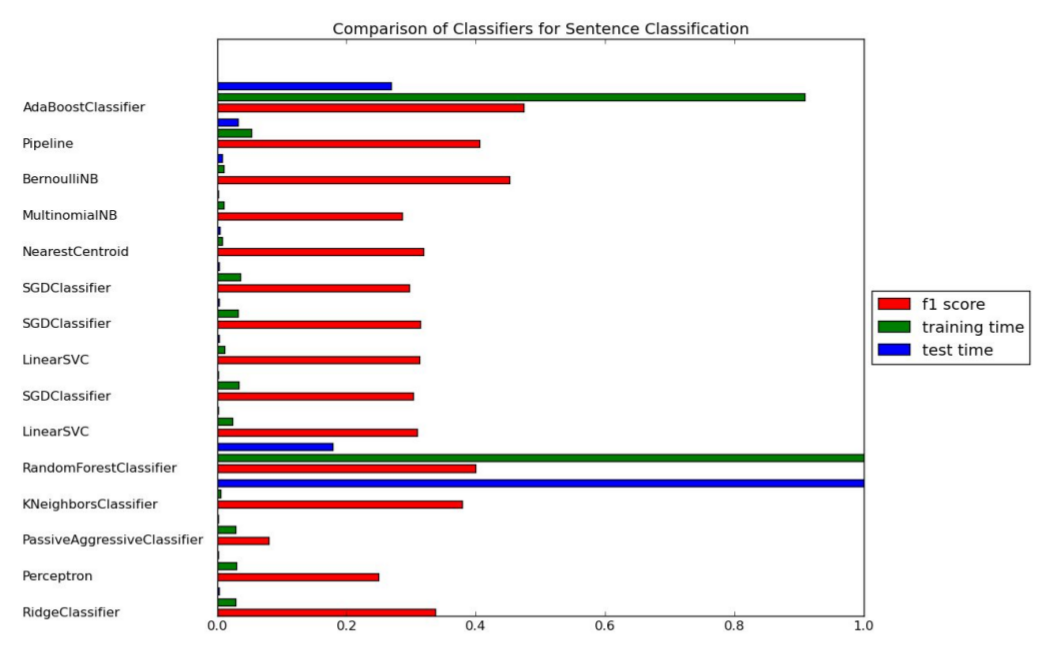
\includegraphics[width=1\textwidth]{scikitlearn.png}}
\caption{Comparison of Classifiers with scikit-learn}
\label{fig:scikit-learn}
\end{figure}

\begin{center}
\captionof{table}{Classification Accuracy of AdaBoost Classifier} \label{tab:adaboost-results} 
\begin{tabular}{ |c||c|c|c| }
	\hline
	\multicolumn{4}{|c|}{AdaBoost Classifier Accuracy} \\
	\hline
	Metric & Knowledge Sentence & General Sentence & Overall \\
	\hline
	Precision & 0.54 & 0.98 & 0.96 \\
	Recall & 0.52 & 0.98 & 0.96 \\
	F1 Score & 0.53 & 0.98 & 0.96 \\
	\hline
\end{tabular}
\end{center}

\subsection{Conditional Random Fields}


\subsubsection*{References}

[1] K. Bowen, B. Brautigam, C. L. Giles, C. Liang, B. Pursel, S. Saul, S. Wang, H. Williams, K. Williams, Z. Wu: BBookX: An Automatic Book Creation Framework. DocEng 2015.

[2] K. Bowen, B. Brautigam, C. L. Giles, C. Liang, B. Pursel, S. Saul, S. Wang, H. Williams, K. Williams, Z. Wu: Concept Hierarchy Extraction from Textbooks. DocEng 2015.

[3] Online Textbooks. {\it National Council of Educational Research and Training.} Web. 5 Nov. 2015. (\url{http://www.ncert.nic.in/ncerts/textbook/textbook.htm})

[4] O. Etzioni, A. Farhadi, H. Hajishirzi, M. J. Seo: Diagram Understanding in Geometry Questions. AAAI 2014.

[5] R. Agrawal, S. Chakraborty, S. Gollapudi, A. Kannan, K. Kenthapadi: Empowering Authors to Diagnose Comprehension Burden in Textbooks. KDD 2012.

[6] R. Agrawal, S. Gollapudi, A. Kannan, K. Kenthapadi: Enriching Textbooks with Images. CIKM 2011. 

[7] R. Agrawal, S. Gollapudi, A. Kannan, K. Kenthapadi: Identifying Enrichment Candidates in Textbooks. WWW 2011.

\end{document}
